\documentclass[12pt,a4paper]{article}
\usepackage[utf8]{inputenc}
\usepackage[T1]{fontenc}
\usepackage{amsmath}
\usepackage{amsfonts}
\usepackage{amssymb}
\usepackage{graphicx}
\usepackage{hyperref}
\usepackage[polish]{babel}
\usepackage{algorithm}
\usepackage{algpseudocode}
\usepackage{booktabs}
\usepackage{float}
\usepackage{subcaption}
\usepackage{changepage}
\usepackage{geometry}
\usepackage{xcolor}

% Marginesy
\geometry{a4paper, margin=2.5cm}

% Fix for Polish algorithm name
\makeatletter
\def\ALG@name{Algorytm}
\makeatother

% Allow algorithms to float but keep them in the same section
% \floatplacement{algorithm}{tbp} % Usunięto globalne ustawienie pływania dla algorytmów

% Make font smaller in algorithm listings
\makeatletter
\algrenewcommand\ALG@beginalgorithmic{\footnotesize}
\makeatother

\title{Hybrydowy Algorytm Ewolucyjny HAE}
\author{Filip Rosiak 151799  \and Eryk Stec 152948}
\date{\today}

\begin{document}

\maketitle

\begin{abstract}
W laboratorium 5 zaprojektowano i zaimplementowano hybrydowy algorytm ewolucyjny (HAE) dla zmodyfikowanego problemu komiwojażera z dwoma rozłącznymi cyklami. Populacja elitarnych rozwiązań (rozmiar 20) podlega steady–state rekombinacji polegającej na usunięciu krawędzi różniących się między rodzicami oraz dodatkowych 20\% wierzchołków, a następnie naprawie heurystyką Ważonego 2-żalu. Przeanalizowano dwa warianty: z lokalnym przeszukiwaniem po rekombinacji (HAE+LS) oraz bez niego (HAE). Wyniki eksperymentów na instancjach \texttt{kroa200} i \texttt{krob200} pokazują, że pominięcie lokalnego przeszukiwania znacząco zwiększa liczbę pokoleń (>300 vs ~95), co przekłada się na lepsze wyniki kosztu (min: 30862/30921; śr.: 31147/31178), przewyższając MSLS, ILS, LNS i LNSa.
\end{abstract}

\section{Opis problemu}
Rozważany problem jest modyfikacją klasycznego problemu komiwojażera. Dany jest zbiór wierzchołków i symetryczna macierz odległości pomiędzy dowolną parą wierzchołków. Zadanie polega na ułożeniu dwóch rozłącznych zamkniętych ścieżek (cykli), każda zawierająca 50\% wierzchołków (jeżeli liczba wierzchołków w instancji nie jest parzysta, to pierwsza ścieżka zawiera jeden wierzchołek więcej), minimalizując łączną długość obu ścieżek.

Do testów wykorzystano instancje \texttt{kroa200} i \texttt{krob200} z biblioteki TSPLib. Są to dwuwymiarowe instancje euklidesowe, gdzie dla każdego wierzchołka podane są dwie współrzędne, a odległość pomiędzy wierzchołkami jest odległością euklidesową zaokrąglaną do liczby całkowitej.

\section{Zaimplementowane algorytmy}
W ramach zadania zaimplementowano i porównano następujące metaheurystyki, oparte na najlepszym algorytmie lokalnego przeszukiwania (LS) z poprzedniego zadania - Candidate Steepest (k=10) z sąsiedztwem Edge Exchange i startem z losowych rozwiązań:

\subsection{Multiple Start Local Search (MSLS)}
Algorytm polega na wielokrotnym uruchomieniu bazowego algorytmu lokalnego przeszukiwania (LS) z różnych, losowo generowanych rozwiązań początkowych. Wynikiem końcowym jest najlepsze rozwiązanie znalezione spośród wszystkich uruchomień LS. W eksperymentach wykonano 200 iteracji (uruchomień LS) dla każdej instancji. Pseudokod przedstawiono w Algorytmie~\ref{alg:msls}.

\begin{algorithm}[H]
\caption{Algorytm: Multiple Start Local Search (MSLS)}
\label{alg:msls}
\begin{algorithmic}[1]
\Require \texttt{instance}, \texttt{base\_local\_search}, \texttt{iterations}
\Ensure \texttt{best\_overall\_solution}
\State \texttt{best\_overall\_solution} $\leftarrow$ \texttt{null}
\State \texttt{min\_cost} $\leftarrow$ $\infty$
\For{$i \leftarrow 1$ to \texttt{iterations}}
    \State \texttt{start\_solution} $\leftarrow$ \texttt{generate\_random\_solution(instance)}
    \State \texttt{current\_solution} $\leftarrow$ \texttt{base\_local\_search(start\_solution, instance)}
    \State \texttt{current\_cost} $\leftarrow$ \texttt{calculate\_cost(current\_solution, instance)}
    \If{\texttt{current\_cost < min\_cost}}
        \State \texttt{min\_cost} $\leftarrow$ \texttt{current\_cost}
        \State \texttt{best\_overall\_solution} $\leftarrow$ \texttt{current\_solution}
    \EndIf
\EndFor
\State \Return \texttt{best\_overall\_solution}
\end{algorithmic}
\end{algorithm}

\subsection{Iterated Local Search (ILS)}
Algorytm rozpoczyna od znalezienia lokalnego optimum za pomocą bazowego LS. Następnie iteracyjnie wykonuje kroki perturbacji i lokalnego przeszukiwania. Perturbacja polega na wprowadzeniu niewielkich, losowych zmian w bieżącym najlepszym rozwiązaniu, aby umożliwić ucieczkę z lokalnego optimum. Po perturbacji ponownie stosowany jest bazowy LS. Nowe rozwiązanie jest akceptowane, jeśli jest lepsze od dotychczas najlepszego. Jako perturbację zaimplementowano \textbf{Perturbację 1}, która wykonuje 10 losowych ruchów (wymiana wierzchołków lub krawędzi) bez sprawdzania ich wpływu na koszt. Warunkiem stopu dla ILS był limit czasowy równy średniemu czasowi wykonania MSLS dla danej instancji. Pseudokod przedstawiono w Algorytmie~\ref{alg:ils}.

\begin{algorithm}[H]
\caption{Algorytm: Iterated Local Search (ILS)}
\label{alg:ils}
\begin{algorithmic}[1]
\Require \texttt{instance}, \texttt{base\_local\_search}, \texttt{perturbation}, \texttt{time\_limit}
\Ensure \texttt{best\_solution}
\State \texttt{start\_solution} $\leftarrow$ \texttt{generate\_random\_solution(instance)}
\State \texttt{best\_solution} $\leftarrow$ \texttt{base\_local\_search(start\_solution, instance)}
\State \texttt{best\_cost} $\leftarrow$ \texttt{calculate\_cost(best\_solution, instance)}
\State \texttt{start\_time} $\leftarrow$ \texttt{current\_time()}
\While{\texttt{current\_time()} - \texttt{start\_time} < \texttt{time\_limit}}
    \State \texttt{current\_solution} $\leftarrow$ \texttt{clone(best\_solution)}
    \State \texttt{perturbation(current\_solution, instance)}
    \State \texttt{current\_solution} $\leftarrow$ \texttt{base\_local\_search(current\_solution, instance)}
    \State \texttt{current\_cost} $\leftarrow$ \texttt{calculate\_cost(current\_solution, instance)}
    \If{\texttt{current\_cost < best\_cost}}
        \State \texttt{best\_solution} $\leftarrow$ \texttt{current\_solution}
        \State \texttt{best\_cost} $\leftarrow$ \texttt{current\_cost}
    \EndIf
\EndWhile
\State \Return \texttt{best\_solution}
\end{algorithmic}
\end{algorithm}

\subsection{Large Neighborhood Search (LNS)}
Podobnie jak ILS, algorytm LNS iteracyjnie modyfikuje rozwiązanie, ale wykorzystuje bardziej radykalną perturbację typu Destroy-Repair. Krok \textbf{Destroy} polega na usunięciu pewnego odsetka (w implementacji 20\%) losowo wybranych wierzchołków z bieżącego rozwiązania. Krok \textbf{Repair} polega na ponownym wstawieniu usuniętych wierzchołków do częściowego rozwiązania za pomocą heurystyki konstrukcyjnej - w tym przypadku zaimplementowano wariant heurystyki \textbf{Ważony 2-żal} (Weighted Regret) do naprawy rozwiązania. Perturbację tę nazwano \textbf{Perturbacja Destroy-Repair (20\%)}. Po naprawie (opcjonalnie) stosowany jest bazowy LS. Zaimplementowano dwie wersje:
\begin{itemize}
    \item \textbf{LNS}: Zastosowanie bazowego LS po kroku Repair.
    \item \textbf{LNSa}: Bez stosowania bazowego LS po kroku Repair (LS stosowane tylko na początku, o ile start był losowy).
\end{itemize}
Warunkiem stopu dla LNS/LNSa był limit czasowy równy średniemu czasowi wykonania MSLS dla danej instancji. Pseudokod przedstawiono w Algorytmie~\ref{alg:lns}.

\begin{algorithm}[H]
\caption{Algorytm: Large Neighborhood Search (LNS)}
\label{alg:lns}
\begin{algorithmic}[1]
\Require \texttt{instance}, \texttt{base\_local\_search}, \texttt{destroy}, \texttt{repair}, \texttt{apply\_ls\_after\_repair}, \texttt{apply\_ls\_to\_initial}, \texttt{time\_limit}
\Ensure \texttt{best\_solution}
\State \texttt{best\_solution} $\leftarrow$ \texttt{generate\_random\_solution(instance)}
\If{\texttt{apply\_ls\_to\_initial}}
    \State \texttt{best\_solution} $\leftarrow$ \texttt{base\_local\_search(best\_solution, instance)}
\EndIf
\State \texttt{best\_cost} $\leftarrow$ \texttt{calculate\_cost(best\_solution, instance)}
\State \texttt{start\_time} $\leftarrow$ \texttt{current\_time()}
\While{\texttt{current\_time()} - \texttt{start\_time} < \texttt{time\_limit}}
    \State \texttt{current\_solution} $\leftarrow$ \texttt{clone(best\_solution)}
    \State \texttt{destroyed\_nodes} $\leftarrow$ \texttt{destroy(current\_solution, instance)}
    \State \texttt{repair(current\_solution, destroyed\_nodes, instance)} \Comment{Używa Weighted Regret}
    \If{\texttt{apply\_ls\_after\_repair}}
        \State \texttt{current\_solution} $\leftarrow$ \texttt{base\_local\_search(current\_solution, instance)}
    \EndIf
    \State \texttt{current\_cost} $\leftarrow$ \texttt{calculate\_cost(current\_solution, instance)}
    \If{\texttt{current\_cost < best\_cost}}
        \State \texttt{best\_solution} $\leftarrow$ \texttt{current\_solution}
        \State \texttt{best\_cost} $\leftarrow$ \texttt{current\_cost}
    \EndIf
\EndWhile
\State \Return \texttt{best\_solution}
\end{algorithmic}
\end{algorithm}

\subsection{Large Neighborhood Search (LNSa)}
\begin{algorithm}[H]
\caption{Algorytm: Large Neighborhood Search (LNSa)}
\label{alg:lnsa}
\begin{algorithmic}[1]
\Require \texttt{instance}, \texttt{base\_local\_search}, \texttt{destroy}, \texttt{repair}, \texttt{apply\_ls\_after\_repair}, \texttt{apply\_ls\_to\_initial}, \texttt{time\_limit}
\Ensure \texttt{best\_solution}
\State \texttt{best\_solution} $\leftarrow$ \texttt{generate\_random\_solution(instance)}
\If{\texttt{apply\_ls\_to\_initial}}
    \State \texttt{best\_solution} $\leftarrow$ \texttt{base\_local\_search(best\_solution, instance)}
\EndIf
\State \texttt{best\_cost} $\leftarrow$ \texttt{calculate\_cost(best\_solution, instance)}
\State \texttt{start\_time} $\leftarrow$ \texttt{current\_time()}
\While{\texttt{current\_time()} - \texttt{start\_time} < \texttt{time\_limit}}
    \State \texttt{current\_solution} $\leftarrow$ \texttt{clone(best\_solution)}
    \State \texttt{destroyed\_nodes} $\leftarrow$ \texttt{destroy(current\_solution, instance)}
    \State \texttt{repair(current\_solution, destroyed\_nodes, instance)} \Comment{Używa Weighted Regret}
    \If{\texttt{apply\_ls\_after\_repair}}
        \State \texttt{current\_solution} $\leftarrow$ \texttt{base\_local\_search(current\_solution, instance)}
    \EndIf
    \State \texttt{current\_cost} $\leftarrow$ \texttt{calculate\_cost(current\_solution, instance)}
    \If{\texttt{current\_cost < best\_cost}}
        \State \texttt{best\_solution} $\leftarrow$ \texttt{current\_solution}
        \State \texttt{best\_cost} $\leftarrow$ \texttt{current\_cost}
    \EndIf
\EndWhile
\State \Return \texttt{best\_solution}
\end{algorithmic}
\end{algorithm}

\subsection{Hybrydowy Algorytm Ewolucyjny (HAE)}
Hybrydowy algorytm ewolucyjny (HAE) łączy operatory rekombinacji z lokalnym przeszukiwaniem na populacji elitarnych rozwiązań. Operator rekombinacji usuwa z jednego rodzica wszystkie krawędzie nie występujące w drugim rodzicu oraz dodatkowo losowo 20\% wierzchołków, po czym naprawa realizowana jest heurystyką Ważony 2-żal (regret), analogicznie jak w LNS. W wersji HAE+LS potomki poddawane są także lokalnemu przeszukiwaniu. Pseudokod przedstawiono w Algorytmie~\ref{alg:hae}.

\begin{algorithm}[H]
\caption{Algorytm: Hybrydowy Algorytm Ewolucyjny (HAE)}
\label{alg:hae}
\begin{algorithmic}[1]
\Require instance, base\_local\_search, pop\_size, min\_diff, time\_limit, with\_local
\Ensure best\_solution
\State Zainicjalizuj populację $P$ rozmiaru \texttt{pop\_size} rozwiązaniami z \texttt{base\_local\_search}
\State \texttt{best\_solution} $\leftarrow$ najlepsze z $P$, \texttt{best\_cost} $\leftarrow$ jego koszt
\State \texttt{start\_time} $\leftarrow$ \texttt{current\_time}()
\While{$\texttt{current\_time}() - \texttt{start\_time} < \texttt{time\_limit}$}
    \State Wybierz losowo dwóch różnych rodziców $p_1, p_2 \in P$
    \State Użyj rekombinacji: usuń krawędzie $p_1$ niewystępujące w $p_2$ oraz dodatkowo 20\% wierzchołków
    \State Napraw wynik heurystyką Ważony 2-żal
    \If{with\_local}
      \State Zastosuj \texttt{base\_local\_search} na potomku
    \EndIf
    \State Oblicz $cost(y)$
    \If{$\neg\exists x\in P:\ \lvert cost(y)-cost(x)\rvert < \texttt{min\_diff}$}
      \State Zamień najgorsze $x\in P$ na $y$, jeśli $cost(y) < cost(x)$
      \If{$cost(y) < \texttt{best\_cost}$}
        \State \texttt{best\_solution} $\leftarrow$ $y$, \texttt{best\_cost} $\leftarrow$ cost(y)
      \EndIf
    \EndIf
\EndWhile
\State \Return best\_solution
\end{algorithmic}
\end{algorithm}

% Opis parametrów użytych w HAE
\paragraph{Parametry HAE}
W naszych eksperymentach przyjęto:
\begin{itemize}
  \item \texttt{pop\_size} = 20: liczba elitarnych rozwiązań utrzymywanych w populacji.
  \item \texttt{min\_diff} = 40: minimalna różnica w koszcie, poniżej której nowy osobnik jest uznawany za zbyt podobny do istniejących i zostaje odrzucony.
\end{itemize}

\section{Wyniki eksperymentów}
Każdy z algorytmów (MSLS, ILS, LNS, LNSa) został uruchomiony 10 razy dla każdej instancji (kroa200, krob200). MSLS wykonywał 200 iteracji bazowego LS (Candidate Steepest k=10). Algorytmy ILS, LNS i LNSa działały przez czas równy średniemu czasowi wykonania MSLS dla danej instancji. Poniżej przedstawiono zagregowane wyniki.

\begin{table}[H]
\centering
\caption{Wyniki algorytmów (średnia, zakres [min - max] kosztu, średni czas, średnia liczba iteracji dla ILS/LNS)}
\label{tab:results}
\resizebox{\textwidth}{!}{%
\begin{tabular}{@{}lccccc@{}}
\toprule
\textbf{Algorytm} & \textbf{Koszt min} & \textbf{Koszt śr.} & \textbf{Koszt max} & \textbf{Czas śr. [ms]} & \textbf{Iteracje śr.} \\
\midrule
\multicolumn{6}{c}{\textbf{Instancja kroa200}} \\
\midrule
MSLS (200 iter.)        & 36327 & 36907.10 & 37331 & 3606.90 & N/A \\
ILS (Perturbacja 1, 10 ruchów)   & 35445 & 36620.80 & 37074 & 3614.90 & 193.4 \\
LNS (Destroy-Repair 20\%)  & 36548 & 36957.00 & 37290 & 3619.80 & 178.4 \\
LNSa (Destroy-Repair 20\%) & 32073 & 32812.20 & 34558 & 3607.70 & 2104.6 \\
HAE+LS (pop=20, min\_diff=40) & 36517 & 36968.60 & 37433 & 3620.20 & 95.0 \\
HAE (pop=20, min\_diff=40) & 30862 & 31147.20 & 31657 & 3611.00 & 313.7 \\
\midrule
\multicolumn{6}{c}{\textbf{Instancja krob200}} \\
\midrule
MSLS (200 iter.)        & 36763 & 37087.80 & 37394 & 3684.20 & N/A \\
ILS (Perturbacja 1, 10 ruchów)   & 35823 & 36848.40 & 37431 & 3696.40 & 199.4 \\
LNS (Destroy-Repair 20\%)  & 36651 & 37132.40 & 37432 & 3691.00 & 181.2 \\
LNSa (Destroy-Repair 20\%) & 32335 & 33275.00 & 34879 & 3684.30 & 2158.2 \\
HAE+LS (pop=20, min\_diff=40) & 36573 & 37313.70 & 37726 & 3697.40 & 98.2 \\
HAE (pop=20, min\_diff=40) & 30921 & 31178.20 & 31383 & 3686.10 & 343.9 \\
\bottomrule
\end{tabular}%
}
\end{table}

\section{Wizualizacje}
Poniżej przedstawiono wizualizacje najlepszych rozwiązań znalezionych przez poszczególne algorytmy dla obu instancji.

\begin{figure}[H]
\begin{adjustwidth}{-1cm}{-1cm} % Dostosuj marginesy dla tej figury
    \centering
    \begin{subfigure}[b]{0.5\textwidth}
        \centering
        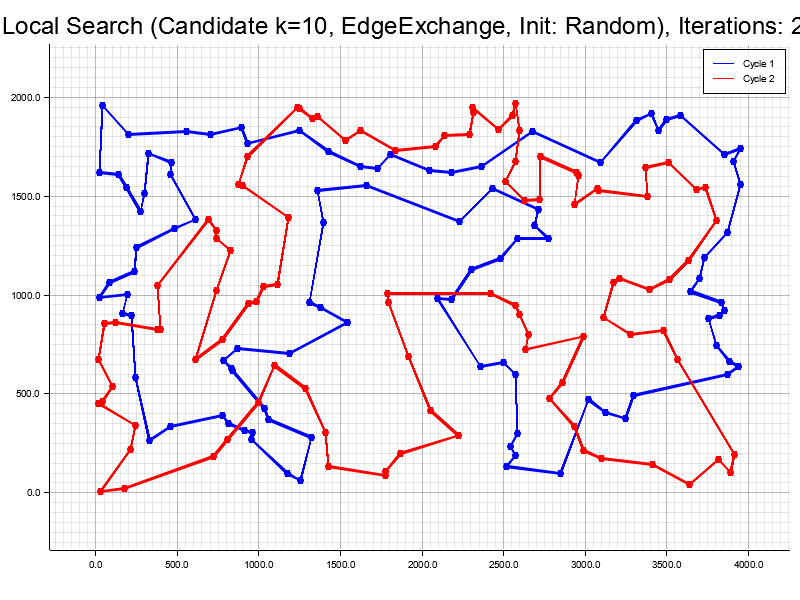
\includegraphics[width=\textwidth]{figures/kroa200_MSLS_Base_Local_Search_Candidate_k_10_EdgeExchange_Init_Random__Iterations_200_.png}
        \caption{kroa200}
    \end{subfigure}%
    \hfill
    \begin{subfigure}[b]{0.5\textwidth}
        \centering
        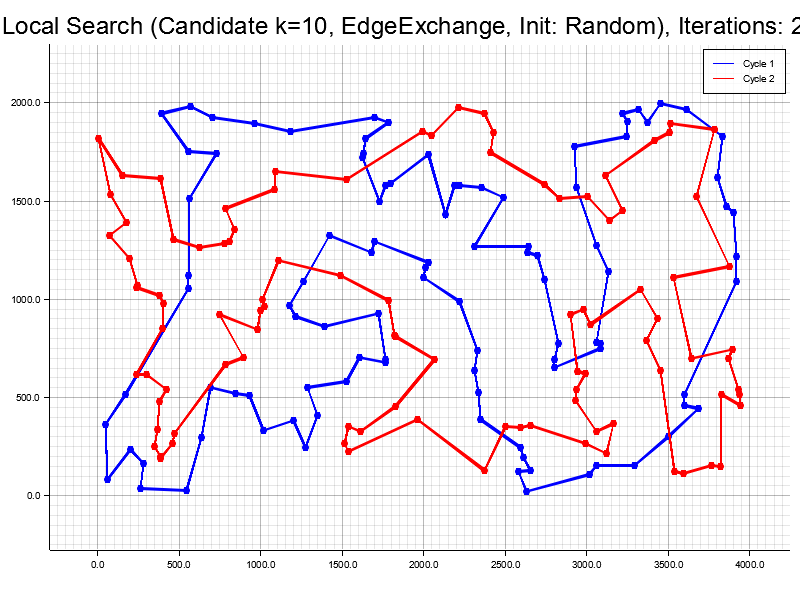
\includegraphics[width=\textwidth]{figures/krob200_MSLS_Base_Local_Search_Candidate_k_10_EdgeExchange_Init_Random__Iterations_200_.png}
        \caption{krob200}
    \end{subfigure}
    \caption{Wizualizacje najlepszych rozwiązań dla MSLS}
    \label{fig:msls}
\end{adjustwidth}
\end{figure}

\begin{figure}[H]
\begin{adjustwidth}{-1cm}{-1cm}
    \centering
    \begin{subfigure}[b]{0.5\textwidth}
        \centering
        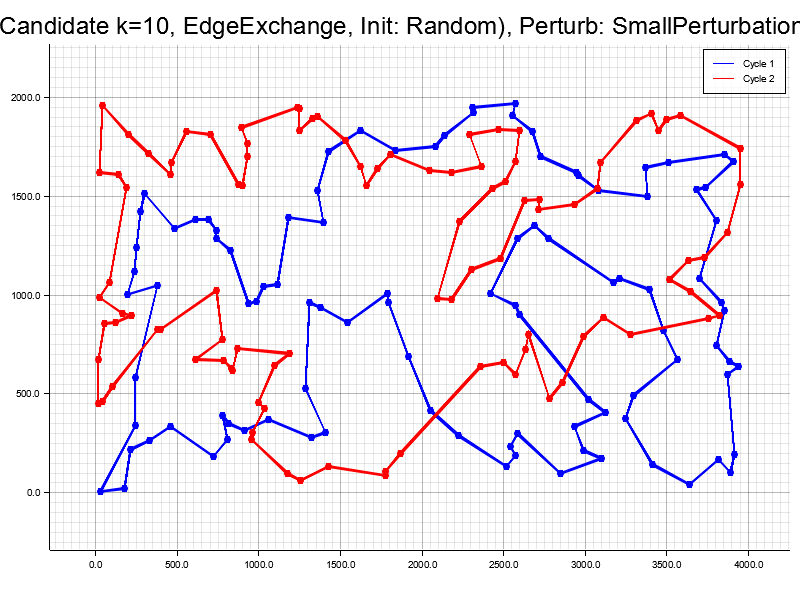
\includegraphics[width=\textwidth]{figures/kroa200_ILS_Base_Local_Search_Candidate_k_10_EdgeExchange_Init_Random__Perturb_SmallPerturbation_n_moves_10_.png}
        \caption{kroa200}
    \end{subfigure}%
    \hfill
    \begin{subfigure}[b]{0.5\textwidth}
        \centering
        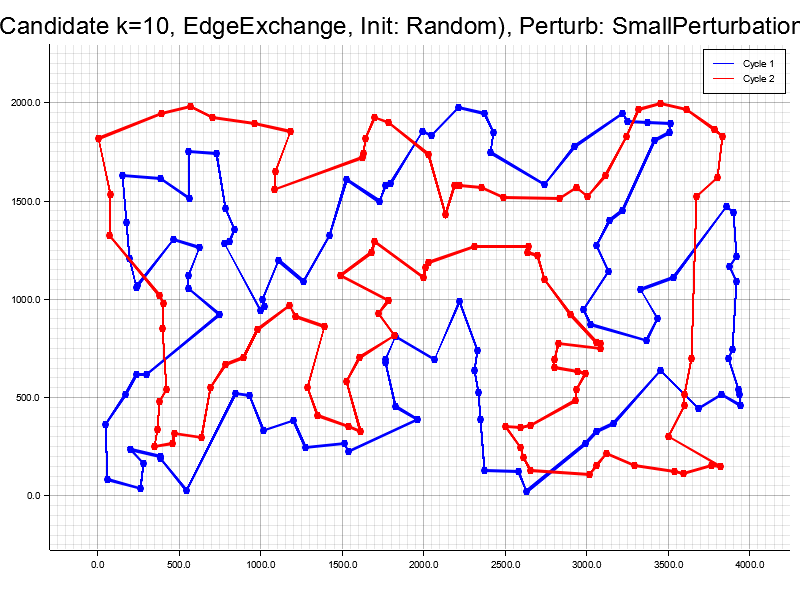
\includegraphics[width=\textwidth]{figures/krob200_ILS_Base_Local_Search_Candidate_k_10_EdgeExchange_Init_Random__Perturb_SmallPerturbation_n_moves_10_.png}
        \caption{krob200}
    \end{subfigure}
    \caption{Wizualizacje najlepszych rozwiązań dla ILS (Perturbacja 1, 10 losowych ruchów)}
    \label{fig:ils}
\end{adjustwidth}
\end{figure}

\begin{figure}[H]
\begin{adjustwidth}{-1cm}{-1cm}
    \centering
    \begin{subfigure}[b]{0.5\textwidth}
        \centering
        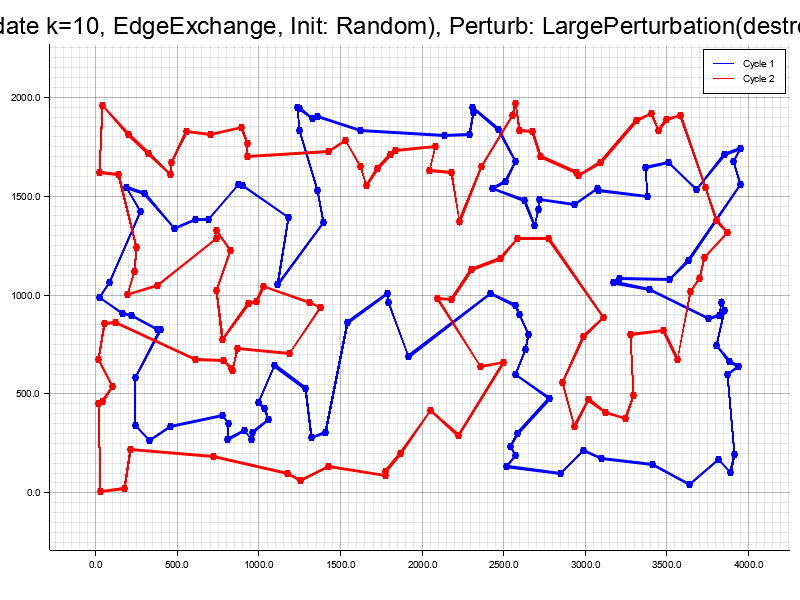
\includegraphics[width=\textwidth]{figures/kroa200_LNS_Base_Local_Search_Candidate_k_10_EdgeExchange_Init_Random__Perturb_LargePerturbation_destroy_0_20__LS_on_Initial_.png}
        \caption{kroa200}
    \end{subfigure}%
    \hfill
    \begin{subfigure}[b]{0.5\textwidth}
        \centering
        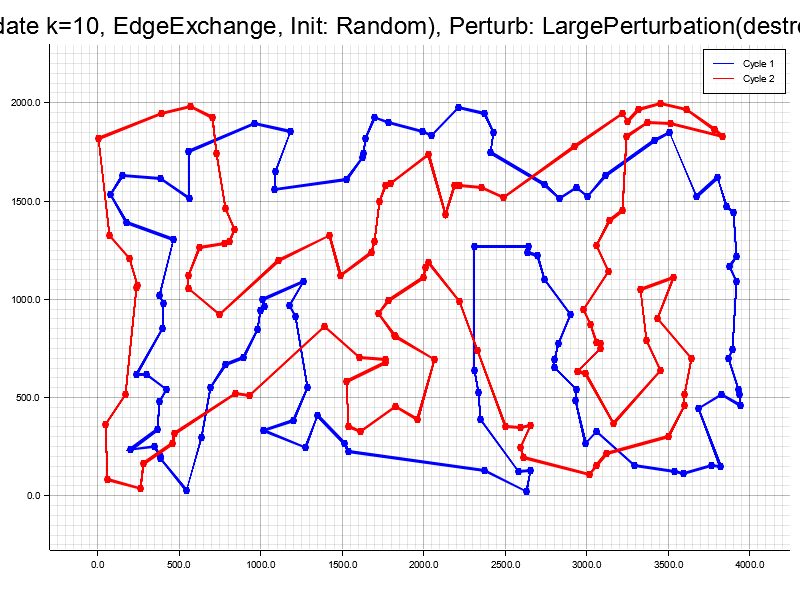
\includegraphics[width=\textwidth]{figures/krob200_LNS_Base_Local_Search_Candidate_k_10_EdgeExchange_Init_Random__Perturb_LargePerturbation_destroy_0_20__LS_on_Initial_.png}
        \caption{krob200}
    \end{subfigure}
    \caption{Wizualizacje najlepszych rozwiązań dla LNS (Destroy-Repair 20\%)}
    \label{fig:lns}
\end{adjustwidth}
\end{figure}

\begin{figure}[H]
\begin{adjustwidth}{-1cm}{-1cm}
    \centering
    \begin{subfigure}[b]{0.5\textwidth}
        \centering
        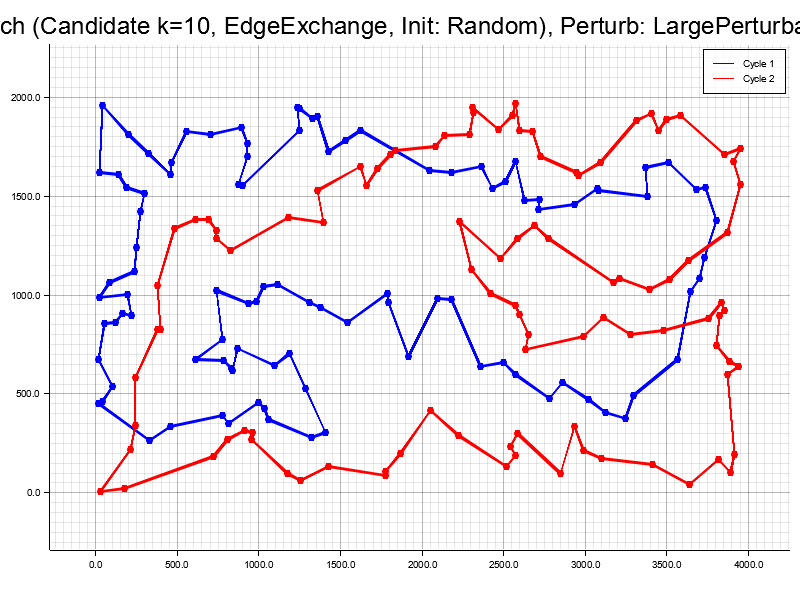
\includegraphics[width=\textwidth]{figures/kroa200_LNSa_no_LS_after_repair__Base_Local_Search_Candidate_k_10_EdgeExchange_Init_Random__Perturb_LargePerturbation_destroy_0_20__LS_on_Initial_.png}
        \caption{kroa200}
    \end{subfigure}%
    \hfill
    \begin{subfigure}[b]{0.5\textwidth}
        \centering
        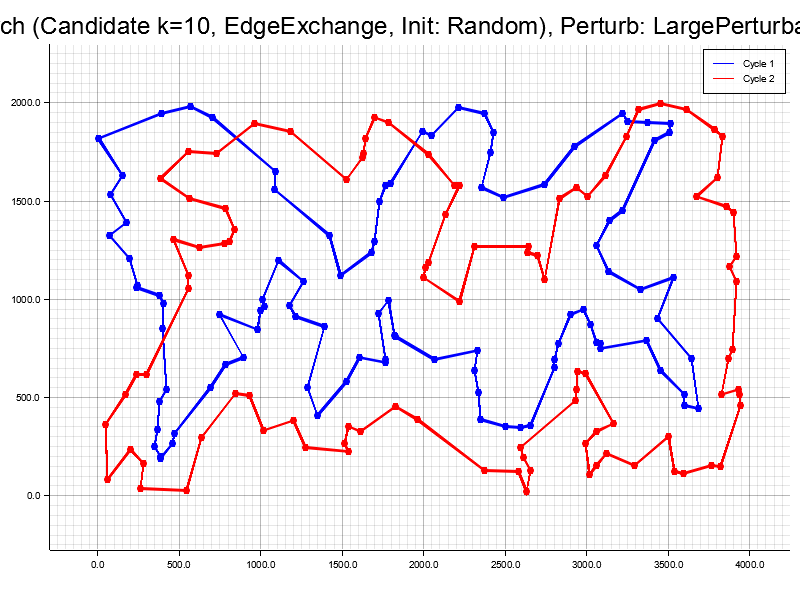
\includegraphics[width=\textwidth]{figures/krob200_LNSa_no_LS_after_repair__Base_Local_Search_Candidate_k_10_EdgeExchange_Init_Random__Perturb_LargePerturbation_destroy_0_20__LS_on_Initial_.png}
        \caption{krob200}
    \end{subfigure}
    \caption{Wizualizacje najlepszych rozwiązań dla LNSa (Destroy-Repair 20\%, bez LS po naprawie)}
    \label{fig:lnsa}
\end{adjustwidth}
\end{figure}

\begin{figure}[H]
\begin{adjustwidth}{-1cm}{-1cm}
    \centering
    \begin{subfigure}[b]{0.5\textwidth}
        \centering
        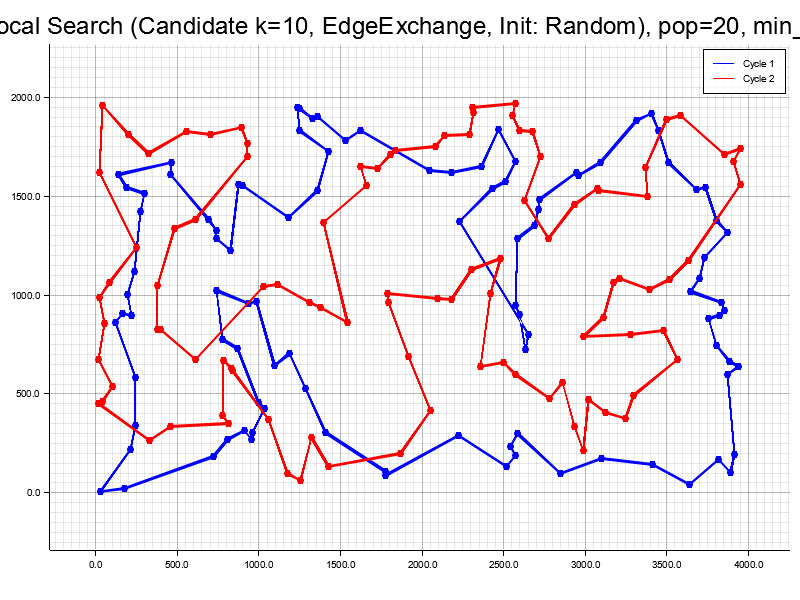
\includegraphics[width=\textwidth]{figures/kroa200_HAE_LS_Base_Local_Search_Candidate_k_10_EdgeExchange_Init_Random__pop_20_min_diff_40_.png}
        \caption{kroa200}
    \end{subfigure}%
    \hfill
    \begin{subfigure}[b]{0.5\textwidth}
        \centering
        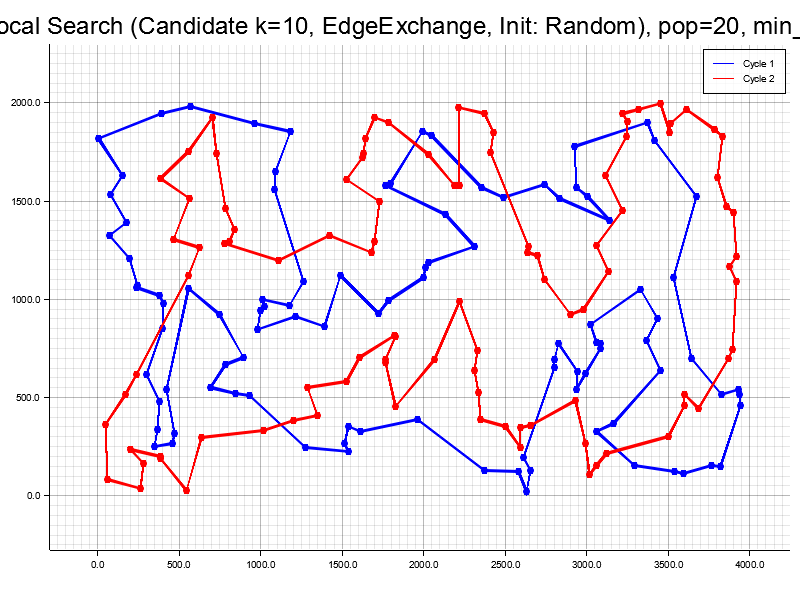
\includegraphics[width=\textwidth]{figures/krob200_HAE_LS_Base_Local_Search_Candidate_k_10_EdgeExchange_Init_Random__pop_20_min_diff_40_.png}
        \caption{krob200}
    \end{subfigure}
    \caption{Wizualizacje najlepszych rozwiązań dla HAE+LS (pop=20, min\_diff=40)}
    \label{fig:hae}
\end{adjustwidth}
\end{figure}

\begin{figure}[H]
\begin{adjustwidth}{-1cm}{-1cm}
    \centering
    \begin{subfigure}[b]{0.5\textwidth}
        \centering
        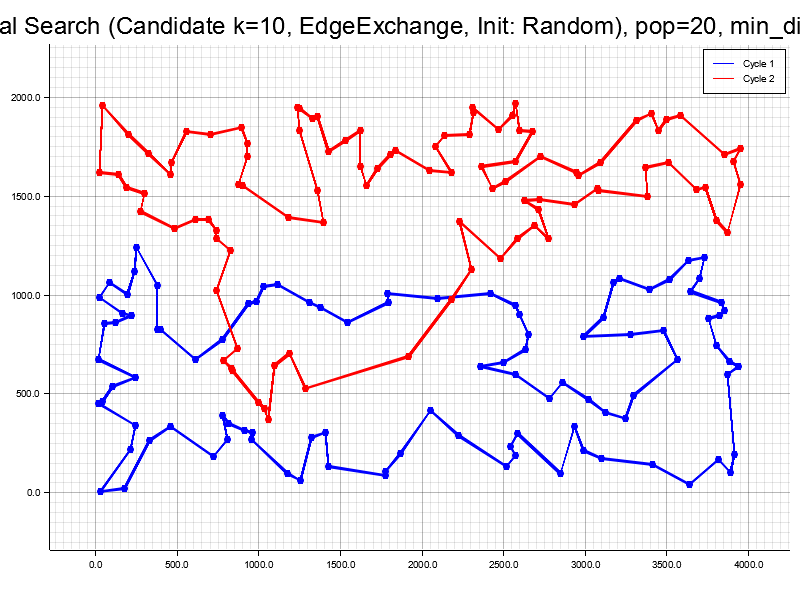
\includegraphics[width=\textwidth]{figures/kroa200_HAE_Base_Local_Search_Candidate_k_10_EdgeExchange_Init_Random__pop_20_min_diff_40_.png}
        \caption{kroa200}
    \end{subfigure}%
    \hfill
    \begin{subfigure}[b]{0.5\textwidth}
        \centering
        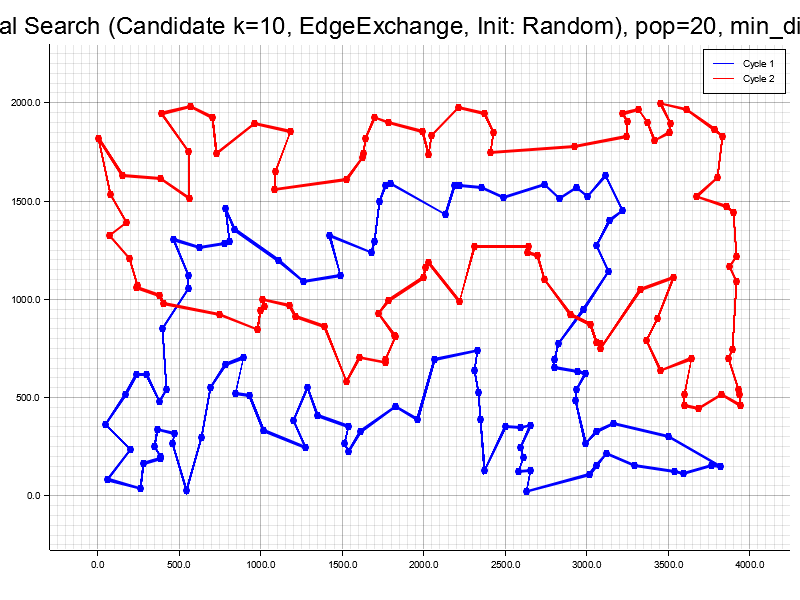
\includegraphics[width=\textwidth]{figures/krob200_HAE_Base_Local_Search_Candidate_k_10_EdgeExchange_Init_Random__pop_20_min_diff_40_.png}
        \caption{krob200}
    \end{subfigure}
    \caption{Wizualizacje najlepszych rozwiązań dla HAE (bez lokalnego przeszukiwania po rekombinacji)}
    \label{fig:hae_nols}
\end{adjustwidth}
\end{figure}

\section{Wnioski}
Na podstawie przeprowadzonych eksperymentów można wyciągnąć następujące wnioski dotyczące zaimplementowanych algorytmów MSLS, ILS i LNS dla rozważanego problemu:

\begin{enumerate}
    \item \textbf{Hybrydowy Algorytm Ewolucyjny ze wzmocnioną LS (HAE+LS):} HAE+LS wykazał mieszane wyniki – dla kroa200 minimalny i średni koszt był nieco wyższy niż w MSLS, a jedynie dla krob200 minimalny koszt był nieznacznie lepszy kosztem wyższej średniej. Algorytm wykonał około 95 pokoleń w zadanym czasie, co wpływało na ograniczoną eksplorację populacji.
    \item \textbf{Hybrydowy Algorytm Ewolucyjny bez LS (HAE):} HAE bez lokalnego przeszukiwania po rekombinacji przeprowadził ponad 300 pokoleń (średnio ok. 314 dla kroa200 i 344 dla krob200) i osiągnął najlepsze wyniki spośród testowanych metod. Minimalny koszt spadł do 30862 (kroa200) i 30921 (krob200), a średnie koszty również były znacznie niższe niż w pozostałych metaheurystykach, co potwierdza korzyść pominięcia kosztownej fazy LS.
\end{enumerate}

Podsumowując, strategie oparte na pomijaniu lokalnego przeszukiwania (LNSa oraz HAE bez LS) pozwoliły na znacznie większą liczbę iteracji i uzyskały najlepsze jakościowo rozwiązania. HAE+LS dostarczał porównywalne wyniki z innymi metaheurystykami, natomiast HAE bez LS osiągnął najlepsze z testowanych minimów kosztów.

\section{Kod źródłowy}
Pełny kod źródłowy implementacji wszystkich algorytmów jest dostępny w repozytorium GitHub:
\url{https://github.com/Veanir/imo-5}

\end{document} 